\subsection{C5 -- Nucleus confinement / neutron stability}\label{app:c5}
\paragraph{Native question.} Does the cited short-window confinement class satisfy the shell-signature, proximity, and $B^*$-dominance conditions required for persistence, or does it cross the transmutation threshold?
\paragraph{Native readout.}
\begin{itemize}
\item cited window $\omega_{\mathrm{nuc}}$
\item structural key \texttt{tetron:3:3:6}
\item frame count / $T_{\mathrm{eval}}=256$ bip
\item weighting policy $w(\kappa)\equiv 1$
\item shell signature
\item proximity criterion
\end{itemize}
\paragraph{Native operator chain.}
\[
e_\alpha,\ e_\Omega,\ f
\;\to\;
b(\kappa)
\;\to\;
H_B
\;\to\;
B^*
\;\to\;
\Lambda_b
\;\to\;
\text{confinement predicate}
\;\to\;
\text{transmutation flag}.
\]
\paragraph{Native output row.}
\begin{center}
\begin{tabularx}{\linewidth}{@{}lXcclll@{}}
\toprule
Row & Structural key & $B^*$ & $\Lambda_b$ & Proximity & Confinement & Transmutation \\
\midrule
C5.A & \texttt{tetron:3:3:6}, $(\lambda=3/2,137,\rho_2,V_4)$ & 137 & 6 & close & confined & 0 \\
C5.B & \texttt{tetron:3:3:6}, $(\lambda=3/2,139,\rho_3,V_4)$ & 139 & 3 & failed & unconfined & 1 \\
\bottomrule
\end{tabularx}
\end{center}
\paragraph{Temporal Conversion Block.} Temporal conversion is a normal chain-rule expansion on the cited native row. This test is retained in native units.
\paragraph{Native figure witness.}
\begin{center}
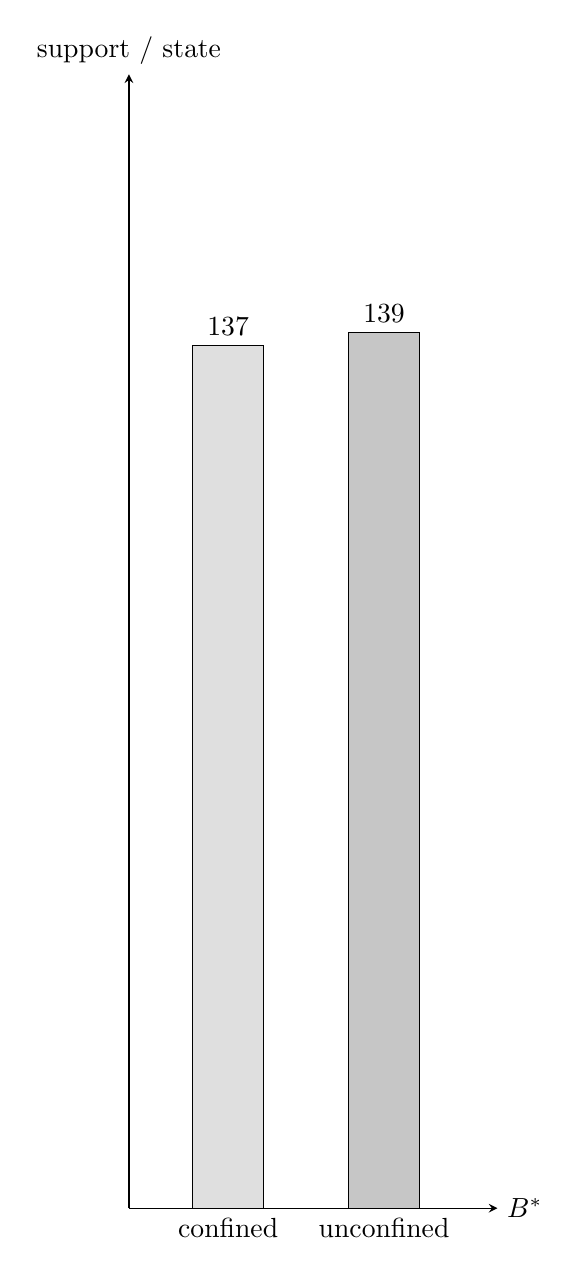
\begin{tikzpicture}[x=1.8cm,y=0.08cm,>=stealth]
\draw[->] (0,0) -- (2.6,0) node[right] {$B^*$};
\draw[->] (0,0) -- (0,180) node[above] {support / state};
\filldraw[fill=gray!25] (0.45,0) rectangle (0.95,137);
\filldraw[fill=gray!45] (1.55,0) rectangle (2.05,139);
\node[below] at (0.7,0) {confined};
\node[below] at (1.8,0) {unconfined};
\node[above] at (0.7,137) {$137$};
\node[above] at (1.8,139) {$139$};
\end{tikzpicture}
\end{center}
\paragraph{Hook / Evidence.} Use the cited confinement, proximity, and transmutation hooks.
